\chapter{Umsetzung}



 

\section{Schnittstelle}

Nachdem in der Transaktion SFP eine Schnittstelle erstellt wurde, werden zunächst die Import-Parameter festgelegt. Die Import Parameter geben an, welche Daten das Druckprogramm an das Formular übergibt. Im Fall der \ac{LLE} sind diese Parameter vom SAP Standard vorgegeben.
Diese Daten beinhalten die Druckparameter, sowie die Informationen, welche den Inhalten des Formulars bestimmen. 

Da die Import Parameter nicht alle benötigten Informationen der \ac{LLE} beinhalten, werden weitere Variablen bei den Globalen Definitionen hinzugefügt. Der Bereich "`Globale Daten"' stellt Variablen zur Verfügung, welche zusätzlich zu den Import Parametern als Datenträger für die Inhalte der \ac{PDF} dienen können. Des Weiteren werden diese Variablen genutzt, um im Laufe der Dokumentenerstellung importierte Daten weiter zu verarbeiten bzw. neue Daten einzulesen.
Die Globalen Definitionen können im Fall der \ac{LLE} aus der alten Smart Form Version übernommen werden, da die selben Variablen Anwendung finden. 

Auf Grund der Tatsache, dass die \ac{LLE} mit einem SAP Standard Druckprogramm erstellt wird, müssen zusätzliche Daten in der Schnittstelle der Adobe \ac{PDF} eingelesen werden. Im Bereich der "`Initialisierung"' wird in der "`Code-Initialisierung"' mit Hilfe von \ac{ABAP}-Code eine Programmlogik erstellt, welche diese Zusatzinformationen von der Datenbank ausliest und in die davor definierten Globalen Variablen schreibt. Hierzu werden Eingabe- und Ausgabe-Parameter definiert. Die Eingabeparameter beinhalten die nötigen Daten, welche in der Code-Initialisierung benutzt werden, um die benötigten Informationen in die Ausgabeparameter zu schreiben. Beispielsweise wird für die \ac{LLE} in der Initialisierung das passende Firmenlogo für die Gesellschaft ausgelesen, welche das Dokument ausstellt. In Abbildung \ref{figCo} ist zu sehen, dass dafür in den Importparametern die \ac{AH} angegeben ist. Die \ac{AH} ist im GTS die eindeutige Einteilung der Gesellschaften und wird deswegen auch im Customizing als Unterscheidungsmerkmal genutzt. Mit Hilfe dieser Information, wird anschließend das zugehörige Firmen Logo ermittelt.

\begin{figure}[ht]
	\centering
	\makebox[\textwidth][c]{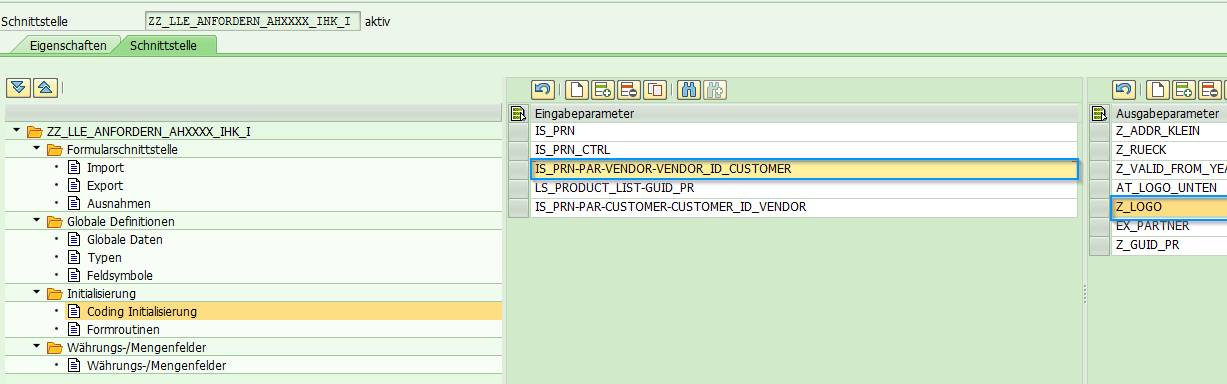
\includegraphics[width=1\textwidth]{img/Init.png}}%		
	\caption{Import- und Export-Parameter in der Code-Initialisierung}
	\label{figCo}
\end{figure}

In diesem Bereich der Schnittstelle ist es ebenfalls möglich, die Daten aus den Importparametern für die Ausgabe aufzubereiten. An vielen Stellen wird in der \ac{LLE} das Jahr abgedruckt, ab dem das Dokument gültig ist. Importiert wird allerdings das gesamte Datum. Um die Verwendung der Jahreszahl zu vereinfachen wird deshalb in der Initialisierung das gewünschte Jahr in eine eigene Variable geschrieben.

Im Fall der \ac{LE} ist die Schnittstelle mit den Globalen Daten und der Code-Initialisierung vollständig. Für andere Formulare gäbe es noch die Möglichkeit, dedizierte Währungsfelder zu definieren. Diese Variablen können den beinhaltenden Wert in jeder gewünschten Währung anzeigen.\footnote{Vgl. \cite{Hauser.2015} S. 138}
Die Schnittstelle kann auch zu späteren Zeitpunkten angepasst werden, falls zusätzliche Variablen benötigt werden oder weitere Logiken in die Initialisierung eingebaut werden müssen.
\FloatBarrier
\section{Formular}
\subsection{Allgemein}


Nach dem Erstellen der Schnittstelle wird das Formular in der Transaktion SFP angelegt. Im Anlageprozess muss unter anderem die zugehörige Schnittstelle angegeben werden. Wie bereits in Kapitel \ref{ch:Aufbau} erläutert, besteht ein Formular im Form Builder aus dem Kontext und dem Layout. Im ersten Teil wird festgelegt, welche der Import- und Globalen-Daten im Layout Bereich für das Dokument zu Verfügung stehen sollen. Zusätzlichen zu diesen Informationen kann die Datenhierarchie bestimmte Bausteine für Texte sowie Adressen beinhalten. Weitere benutzbare Funktionen wie beispielsweise eine Schleifenfunktion dienen dazu, die übertragenen Daten aus der Schnittstelle darzustellen.

Um zu vermeiden, dass Daten und Variablen ungenutzt im Kontext miteinbezogen werden, ist eine gute Vorgehensweise, den Kontext nach Bedarf in mehreren Iterationen mit benötigten Elementen aufzufüllen.

\subsection{Anschreiben der \acs{ABB}}
\subsection{Anschreiben der \acs{LLE}
	
	
		
	Im Fall der \ac{LLE} gibt es verschiedenen Informationen welche im Adresskopf angezeigt werden müssen. Ein Block beinhaltet neben den Kontaktdaten zusätzlich noch weitere Informationen zum Dokument, wie beispielsweise der \ac{LLE}-Nummer. Eine anderer Teil des Adresskopfes besteht nur aus dem Standard Name/Straße/Ort Block.
	Für die individuellen Adressfelder wird die Methode mit den Fließfeldern angewandt. In Abbildung \ref{figAdr}
	ist zu sehen, dass so die Anforderungen am besten umgesetzt werden können.
	
	\begin{figure}[ht]
		\centering
		\makebox[\textwidth][c]{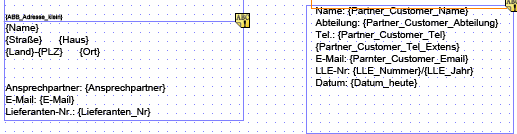
\includegraphics[width=1\textwidth]{img/Adr.png}}%		
		\caption{Adresskopf mit Fließfeldern}
		\label{figAdr}
		
	\end{figure}
	
	Für den Standardadresskopf wird die Adressknoten Variante verwendet. Somit wird zunächst im Kontextbereich ein Adressknoten erstellt, welcher die Adressnummer der zugehörigen Adresse beinhaltet. Zusätzlich wird eine Variable angegeben, welche das Absender Land beinhaltet, da davon das Ausgabelayout abhängig ist.
	
	Die Position der Adressköpfe wird festgelegt und ist für jede Gesellschaft gleich. Diese Vereinheitlichung führt zu einer höheren Übersichtlichkeit des Formulars bei zukünftigen Anpassungen. Der Inhalt der Adressen ist ebenfalls ein Zusammenschluss der vielfachen Varianten der früheren Version des Dokumentes.
	
	
	\FloatBarrier
\subsection{Materialliste}




Für die Materialliste wird zunächst der Kontextbereich des Formulars erweitert. Es wird ein Knotenpunkt in Form eines Ordners erstellt, welcher die Elemente der Tabelle beinhalten soll. In diesem Ordner wird anschließend eine Schleife angelegt. Im Fall der \ac{LLE} soll jeder Eintrag der Materialliste im Layout angezeigt werden. Demnach wird in der angelegten Schleife die Materialliste angegeben. Innerhalb der Schleife wird dann eine Zeile dieser Tabelle als Struktur eingetragen. Diese Zeile wird beim erstellen des Formulars mit jedem Eintrag der Materialliste gefüllt. Zusätzlich wird eine Programmknoten in die Schleife eingefügt. Dieser \ac{ABAP}-Code wird ebenfalls bei jedem Durchlauf der Schleife erneut ausgeführt. Diese Programmlogik wird benötigt um Teile der Materialliste für die Darstellung auf dem Formular aufzubereiten.

Nachdem der Kontext Bereich angepasst wurde, wird anschließend die Tabelle im Layout eingebaut. Zunächst wird mit Hilfe des Tabellen-Assistenten des \ac{ALCD} eine Tabelle mit 7 Spalten erstellt. Diese Tabelle wird in einem Teilformular umschlossen. Anschließend wird in der Objekt Palette der Tabelle der Seitenumbruch freigegeben. Des Weiteren wird in der Palette der Kopfzeile eingestellt, dass der Kopf auf jeder umgebrochenen neuen Seite erneut angezeigt werden soll. Um einen Seitenumbruch in Mitten einer Zeile zu vermeiden, wird für die Zeilen ein Umbruch in der Palette nicht erlaubt. 

Nachdem noch weitere Layout Einstellungen, wie Zeilenhintergründe und Größe, vorgenommen wurden, wird anschließend der Inhalt der Tabelle festgelegt. Wie in Abbildung \ref{figTab} zu sehen ist, werden die Daten der Tabelle ebenfalls mit Fließfeldern abgebildet. Aufgrund der vorher festgelegten Schleife wird somit für jeden Eintrag der Materialliste eine neue Zeile ausgegeben.

\begin{figure}[ht]
	\centering
	\makebox[\textwidth][c]{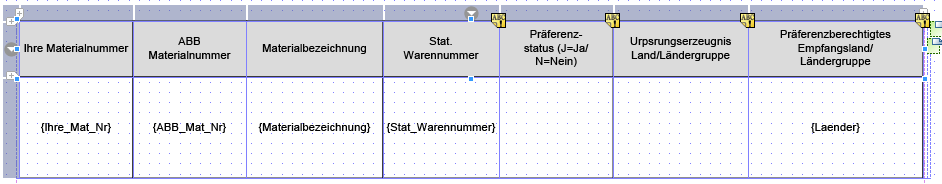
\includegraphics[width=1\textwidth]{img/Tabelle.png}}%		
	\caption{Materialliste mit Fließfeldern}
	\label{figTab}
	
\end{figure}

Um das Layout der Seiten nach einem Umbruch festlegen zu können, wird abschließend in der Objekt-Palette der Seite festgelegt, welche Masterseite für diese Seiten benutzt werden soll. Ansonsten würde die Tabelle auf einer leeren neuen Seite umformatiert weitergeführt werden.

\FloatBarrier
\subsection{Legende}


\section{Abschluss der Umstellung}




\FloatBarrier
\subsection{Master- und Design-Seiten}
\label{ch:tab}

Den Grundstein des Layouts bilden die Masterseiten. Zunächst wird für jede benötigte Seite eine Masterseite erstellt. In Abbildung \ref{figLLE} ist der Aufbau der \ac{LLE} dargestellt.

\begin{figure}[ht]
	\centering
	\makebox[\textwidth][c]{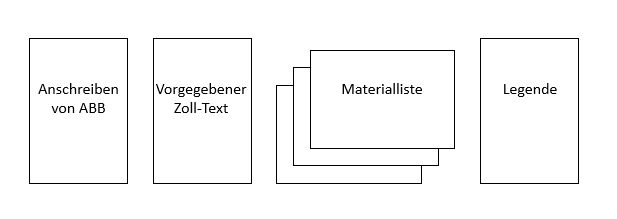
\includegraphics[width=1\textwidth]{img/LLE.png}}%		
	\caption{Aufbau der Lieferantenerklärung}
	\label{figLLE}
	
\end{figure}

Das zweiseitige Anschreiben, der Zoll Text und die Legenden werden im Hochformat und die Materiallisten im Querformat ausgegeben. Die beiden Listen können beliebig lang sein und müssen auf neue Seiten mit dem selben Layout umgebrochen werden.
Die Nummerierung des Dokumentes wird ebenfalls über die Meisterseiten gesteuert. Das Anschreiben soll nicht in die Seitenzahlen miteinbezogen werden, dementsprechend wird in der Objekt Palette dieser Masterseiten eingestellt, dass diese nicht in die Nummerierung aufgenommen werden. Um den Inhaltsbereich der Seiten positionsweise festzulegen, wird auf den Meisterseiten ein Bereich definiert, welcher die Proportionen des Inhaltes eingrenzt. 
  
In der Design Ansicht wird für jede Masterseite auch eine Inhaltsseite eingefügt. Diesen Inhaltsseiten wird in der Objekt Palette bei "`Platzierung"' dem zugehörigen Inhaltsbereich einer Masterseite zugewiesen. Diese Zuweisung führt dazu, dass das Layout der Masterseite und der Inhaltsbereich übernommen wird.

Für die Materiallisten wird in der Objekt-Palette der Inhalt auf "`Textfluss"' umgestellt. Diese Einstellung führt dazu, dass der Inhaltsbereich sich mit dem Inhalt vergrößert, falls mehr Platz nötig sein sollte. Da die Listen über mehrere Seiten abgebildet werden, wird außerdem der Haken in der Palette gesetzt, dass ein Seitenumbruch im Inhalt zugelassen wird.




\FloatBarrier
\section{Einzelne Felder}

Nachdem die Grundstruktur des Formulars mit den Master- und Design-Seiten feststeht wird der Inhalt eingefügt.
Zunächst werden die großen Textfelder für das Anschreiben, sowie die Zolltexte erstellt. Dafür kann die Bibliothek des \ac{ALCD} benutzt werden. Die Felder werden mit Hilfe der Layout-Palette positioniert. Diese Palette dient als Steuerung für alle Layout-Einstellungen eines Elements im \ac{ALCD}. Die Texte werden anschließend in die neu erstellten Felder eingefügt. 

Dynamische Inhalte in Texten können über sogenannte Fließfelder gesteuert werden. Im Fall der \ac{LLE} muss des Öfteren das aktuelle Datum bzw. das Jahr, ab welchem das Dokument gültig ist, in den Text eingefügt werden.
Ein solches Fließfeld wird dementsprechend in den Text eingefügt. Über die Objekt-Palette wird dem Fließfeld eine Datenbindung eingestellt. Diese Bindung verweist auf eine Variable, welche im Kontextbereich definiert wurde. Zum Zeitpunkt des Druckes des Dokumentes wird das Fließfeld durch den Inhalt der verbundenen Variable ersetzt. Der Text um das Feld herum passt sich an die Größe des Inhalts an. In Abbildung \ref{figdt} ist zu sehen, dass Fließfelder im Text durch geschweifte Klammern gekennzeichnet sind.

\begin{figure}[ht]
	\centering
	\makebox[\textwidth][c]{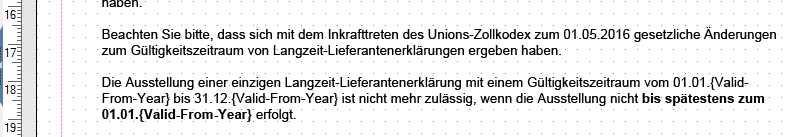
\includegraphics[width=1\textwidth]{img/fliesfeld.png}}%		
	\caption{Fließfelder im Text}
	\label{figdt}
	
\end{figure}



\FloatBarrier



\section{Dynamische Anzeige}
\label{ch:Dyn}

Da die \ac{LLE} von unterschiedlichen Gesellschaften genutzt wird ist es notwendig, dass das Formular sich den jeweiligen Gesellschaften anpasst. Diese Anforderung wird umgesetzt, indem Felder des Formulars, welche im Kontext Bereich definiert wurden, nur unter bestimmten Bedingungen angezeigt werden. Dafür wird ebenfalls im Kontext für die relevanten Felder die Bedingung angelegt, dass sie nur gültig sind wenn eine bestimme \ac{AH} Nummer als Absender eingetragen ist. Anschließend werden im Layout die unterschiedlichen Felder an die bestimmten Positionen gestellt, an welchen der dynamische Inhalte angezeigt werden soll. 

Aufgrund von gesellschaftsspezifischen Anforderungen müssen teilweise Logos an festgelegten Positionen angezeigt werden. Eines dieser festgelegten Logos überdeckt dadurch einen Teil des Adresskopfes, welcher in der alten Version der \ac{LLE} für diese Gesellschaft nicht angezeigt wurde. Um dieses Problem zu lösen wird diesem Teil der Adressen ebenfalls eine Bedingung eingetragen, um die Ausgabe bei dieser Gesellschaft zu unterbinden.  

Die Anzeige der Logos wird mit Hilfe von Grafikelementen umgesetzt, welche im Kontext definiert werden können. Diese Elemente funktionieren in einer ähnlichen Weise wie die Adressfelder. Durch die Zuweisung einer Variablen, die den Namen des Logos beinhaltet, wird das Bild automatisch aus der Datenbank ausgelesen. Diese Methode funktioniert ausschließlich dann, wenn die benötigten Grafiken auf der Datenbank abgespeichert sind.

Zusätzlich zu den bedingten Inhalten muss das Formular in der Lage sein, auf den dynamischen Inhalt reagieren zu können. Im Fall der \ac{LLE} ist ein dynamischer Inhalt die Materiallisten. Da diese Listen eine beliebige Länge erreichen können ist es notwendig, dass die Ausgabe durch automatische Seitenumbrüche trotzdem funktioniert. Wie bereits in Kapitel \ref{ch:tab} beschrieben ist die durch die Textfluss Option gelöst.
Die Seitenzahlen des Formulars müssen ebenfalls dynamisch an den Inhalt angepasst sein.

\FloatBarrier

\section{Ausgabe}

Nach der Fertigstellung des Formulars gilt es, die neue PDF Form im Customizing jeder Gesellschaft zuzuordnen. Nachdem diese Einstellung vorgenommen wurde, kann nun die \ac{LLE} in Form einer PDF ausgegeben werden. Weitere Anpassungen sind nicht nötig.


